\chapter{Small Angle X-ray Scattering Tensor Tomography}
\label{chap:SAXSTT}

Small Angle X-ray Scattering Tensor Tomography is a characterisation technique where the aim is to reconstruct the reciprocal space map in each voxel of a three-dimensional sample
that holds nanostructures with anisotropic electron distribution. Essentially, the technique is computed tomography, but with X-ray scattering patterns instead of X-ray absorption measurements.
Using the scattering patterns obtained from different polar and azimuthal angles, the goal is to determine a tensor for each voxel in the sample,
so that the estimated orientational scattering patterns are in close resemblance to the measured scattering.
Therefore, the optimisation task is closely related theoremautorefname maximum likelihood estimation. The converged model with the minimal error is most likely very similar to the attributes of the physical sample.
In this way, one can map the orientation and the anisotropy of the nanostructures throughout the three-dimensional bulk sample.

\section{X-ray Pencil Beam} % Or in experimental setup. Define brilliance
The first crucial component of SAXSTT is the quality of the X-ray beam.
Obviously, more photons increase the signal-to-noise ratio, and thus the resolution of the electron density distribution is improved.
Moreover, the voxel size is determined by the size of the X-ray beam, where a focused beam results in higher resolution of the reconstructed tensors at the cost of reconstruction time.
Finally, the most consistent scattering occurs when the X-ray beam is almost purely monochromatic, meaning that the spectral bandwidth is narrow.
All these properties are defined by the brilliance of the beam, given as
\begin{equation}\label{eq:brilliance}
    Brilliance = \frac{Photons/second}{\left( mmrad \right)^{2} \left( mm^{2} \right) \left( 0.1\% BW \right).},
\end{equation}
where $BW$ is a commonly used abbreviation for spectral bandwidth \cite{mcmorrow2011elements}.

\section{Experimental Setup}
The experimental part of the SAXSTT process consists of collecting a series of two-dimensional SAXS patterns from different orientations $\left(\alpha,\beta\right)$.
Figure \ref{fig:orientations} shows the definition of the angles $\alpha$ and $\beta$. % Fix. 

\begin{figure}[h!]
    \centering
    %\includegraphics[width = 0.4\textwidth]{../XRD_CT/Figures/Coord_system.png} %RSD: Pdf becomes wrong
    \includesvg[width=0.4\textwidth]{../XRD_CT/Figures/Coord_system.svg}
    \caption{Definition of the polar angle $\alpha$ and azimuthal angle $\beta$, used to express the orientation of the sample.}
    \label{fig:orientations}
\end{figure}

In order to reconstruct tensors, the sample must be rotated around two axes of rotation, unlike conventional CT which only requires one \cite{liebi2018small}.
The synchrotron beam scans across the sample in a raster pattern for each orientation, and collects the combined scattering intensity for each sector of the diffractogram, respectively.
Figure \ref{fig:experimental_setup} shows the experimental setup of a given SAXSTT experiment for a single orientation and at a single scanning point $(\alpha, \beta,x,y)$.

\begin{figure}
    \centering
    \includesvg[width=0.8\textwidth]{../XRD_CT/Figures/SAXSTT_test.svg}
    %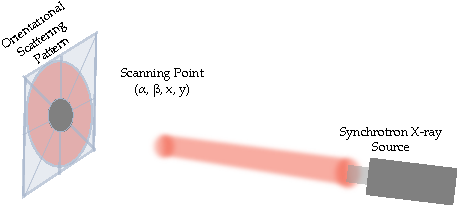
\includegraphics[width = 1\textwidth]{Figures/SAXSTT_annotated.pdf}
    \caption{Experimental setup of a SAXSTT experiment. The beam canon represents the synchrotron beam. The cube represents a single row of voxels in the sample.
        The scattering intensity from eight sectors of the diffractogram is collected for each scanning point $(\alpha, \beta,x,y)$.
        Due to uniaxial symmetry, only half of the circular diffractogram needs to be sampled. The half-circle is partitioned into 8 sector, which means that the entire diffractogram is divided into 16 sectors of 22.5 degrees.}
    \label{fig:experimental_setup}
\end{figure}

%Figure of scanning orientations?


\section{Modelling of Anisotropic Scattering}
The coordinate systems used in this Thesis follow the convention of the article "Small-angle X-ray scattering tensor tomography:
model of the three-dimensional reciprocal-space
map, reconstruction algorithm and angular
sampling requirements" \cite{liebi2018small}.
The reciprocal space map of a voxel is denoted $\vectorBU{\widehat{R}}(\vectorBU{r'}, \vectorBU{q'})$,
where $\vectorBU{r'}$ and $\vectorBU{q'}$ are the position and scattering vector in the object-coordinate system, respectively.
Transformation from the lab-coordinate system $\vectorBU{a}$ to the object-coordinate system $\vectorBU{a'}$ for a given property $\vectorBU{a}$
is given by the applying the rotation matrix $\vectorBU{R}_{n}^{exp}$ of the given projection $n$ with orientation $\left(\alpha,\beta\right)$.
Note that the properties often are higher order tensors, in which case the rotation matrix is applied so-called "page-wise".

% Fig to show alpha and beta. Thinking simple sphere with dots. 

One choice of representing the reciprocal space map is to model the form factor as a linear combination of spherical harmonics functions.
The reciprocal space map is then,
as given in Equation \eqref{eq:scattering_intensity_classical}:

\begin{equation}\label{eq:reciprocal_space_map}
    \vectorBU{\widehat{R}}(\vectorBU{r'}, \vectorBU{q'}) = \left\| \sum_{l, m=0} \vectorBU{a}_{l}^{0}(\vectorBU{r'}, q') \vectorBU{Y}_{l}^{0} \{ \Theta(\vectorBU{r'}, q'), \Phi(\vectorBU{r'}, q') \} \right\|^{2}.
\end{equation}

Equation \eqref{eq:reciprocal_space_map} only sums over the spherical harmonics functions $\vectorBU{Y}_{l}^{0}$ and coefficients $\vectorBU{a}_{l}^{0}(\vectorBU{r'}, q')$ with $m=0$, since the nanostructures are assumed to have uniaxial symmetry.
As shown in Figure \ref{fig:spherical_harmonics}, the increasing even $l$-values of the spherical harmonics functions $\vectorBU{Y}_{l}^{0}$ correspond to higher degree of uniaxiality.

\begin{figure}[h!]
    \centering
    \includesvg[height=0.4\textwidth]{../XRD_CT/Plotting/plots/sph_harm_samples.svg}
    \caption{Spherical harmonics functions $\vectorBU{Y}_{l}^{0}$ with increasing even $l$-values.
        %RSD: Anything to say about the colours?
    }
    \label{fig:spherical_harmonics}
\end{figure}


Moreover, $q' = |\vectorBU{q'}|$ is the magnitude of the reciprocal vector $\vectorBU{q'}$, and $\Theta(\vectorBU{r'}, q')$ and $\Phi(\vectorBU{r'}, q')$ are the polar and azimuthal angles of the spherical harmonics function.
These angles may implicitly be defined by a series of coordinate transformations:

\begin{equation}\label{eq:coordinate_transformations}
    \begin{pmatrix}
        sin \Theta cos \Phi \\
        sin \Theta sin \Phi \\
        cos \Theta
    \end{pmatrix}
    = \vectorBU{R}^{str} \vectorBU{R}_{n}^{exp}
    \begin{pmatrix}
        sin \theta cos \phi \\
        sin \theta sin \phi \\
        cos \theta
    \end{pmatrix},
\end{equation}
\noindent
where $\vectorBU{R}^{str}$ is the rotation of the zenith of the spherical harmonics function in each voxel. The preferred orientation is parameterised by $(\theta_{op}, \varphi_{op})$.
The input is the spherical position coordinates in the lab-coordinate system $\vectorBU{r}$.
The rotation matrices in Equation \eqref{eq:coordinate_transformations} are defined as follows:
\begin{equation}
    \begin{split}
        \vectorBU{R}^{str}(\vectorBU{r'}) &=
        \begin{pmatrix}
            \costhetaop \cosphiop & \costhetaop \sinphiop & -\sinphiop  \\
            -\sinphiop            & \cosphiop             & 0           \\
            \sinthetaop \cosphiop & \sinthetaop \sinphiop & \costhetaop
        \end{pmatrix}\\
        \vectorBU{R}_{n}^{exp} &=
        \begin{pmatrix}
            \cos \beta & \sin \alpha \cos \beta & -\cos\alpha \sin\beta \\
            0          & \cos \alpha            & \sin \alpha           \\
            \sin\beta  & - \sin\alpha \cos\beta & \cos\alpha \cos\beta
        \end{pmatrix}
    \end{split}
\end{equation}

Alternatively, one could model the form factor using a function where one parameter controls the amplitude, and the other controls the degree of uniaxiality, for instance
\begin{equation}\label{eq:exp_sin_squared}
    \vectorBU{\widehat{R}}(\vectorBU{r'}, \vectorBU{q'}) = A^{2} \exp\{-B \sin^{2}\left( \Theta\right) \},
\end{equation}
with the resulting shape in threedimensional space shown in Figure \ref{fig:exp_sin_squared}.

\begin{figure}
    \centering
    \includesvg[height=0.4\textwidth]{../XRD_CT/Plotting/plots/exp_sin_samples.svg}
    \caption{The function in Equation \eqref{eq:exp_sin_squared} for some sets of parameters.}
    \label{fig:exp_sin_squared}
\end{figure}

There are a total of four parameters to optimise in Equation \eqref{eq:exp_sin_squared}: $A$, $B$, $\theta_{op}$, and $\varphi_{op}$.
In contrast, six parameters per voxel need to be optimised in Equation \eqref{eq:reciprocal_space_map},
$a_{0}$, $a_{2}$, $a_{4}$, $a_{6}$, $\theta_{op}$, and $\varphi_{op}$.
Moreover, the alternative representation provides with a continuous degree of uniaxiality
as opposed to the finite number of orders of spherical harmonics functions that can be included.
However, Equation \eqref{eq:reciprocal_space_map} is more general and can be used to model a linear combination of isotropic and uniaxial intensities.
The shape of the function for some sets of parameters is shown in Figure \ref{fig:exp_sin_squared}.


\section{Optimisation Algorithm}

SAXSTT is approximately a Maximum Likelihood Estimation that can utilise gradient descent for optimisation, as mentioned in Chapter \ref{ch:optimisation}.
The forward pass of SAXSTT is to calculate the resulting SAXS patterns from having the currently estimated model.
Then, the error between the calculated and measured SAXS patterns can be calculated.
In terms of cost function expressions, there exist many options, and the expression used by Liebi \cite{liebi2018small} is:
\begin{equation}
    \epsilon_{q} = 2 \sum_{n, x, y, \phi} \omega_{n}(x,y,q,\phi) \left\{ \left( \widehat{I}_{n}(x,y,q,\phi) \right)^{\frac{1}{2}}  -  \left( \frac{ I_{n}(x,y,q,\phi) }{T_{n}(x,y)} \right)^{\frac{1}{2}} \right\}^{2},
\end{equation}
\noindent
where the respective parts of the expression are a binary mask $\omega$, the calculated SAXS patterns $\widehat{I}_{n}$, the measured SAXS patterns $I_{n}$, and the transmission intensity $T_{n}$.
The latter accounts for absorption, which was another phenomenon, in addition to scattering, occurring when X-rays interact with matter,
as seen in Equation \eqref{eq:qm_interaction_Hamiltonian} in Chapter \ref{ch:scattering}.

The calculated SAXS patterns $\widehat{I}_{n}$ can be estimated in a number of ways.
However, it is generally an interpolation of the estimated reciprocal space map model $\vectorBU{\widehat{R}}$ from the given projections.
Since the SAXS patterns are projections, each SAXS projection $n$ can be expressed as a sum along the X-ray beam,
\begin{equation}\label{eq:SAXS_intensity}
    \widehat{I}_{n}(x,y,q,\phi) = \sum_{z} \reciprocalspacemap.
\end{equation}

Additional effort is recommended to ensure that the Maximum Likelihood Estimation is converging towards the correct solution.
A separation of the optimisation into four steps was performed by Liebi \cite{liebi2018small} to ensure that the model was near convergence when optimising all parameters at once.
Therefore, the isotropic component $a_{0}$ is optimised first, followed by the preferred orientation $(\theta_{op}, \varphi_{op})$. In the second step, a guess of the uniaxial compontents has to be made.
Following this, the uniaxial components $a_{l}$ are optimised.
This allows the final optimisation to converge to a lower error value than if only one full optimisation were to be performed.


\section{Degree of Uniaxiality} %RSD: Or Anisotropy?

A common measure for the degree of uniaxiality is needed to quantify the results of SAXSTT.
The Hermans order parameter is common for describing the degree of uniaxiality \cite{yoshiharu1997cellulose}.
The order parameter $S$ is defined as,
\begin{equation}
    S = \frac{1}{2} \left( 3 <\cos^{2} \Theta> - 1 \right),
\end{equation}.
\noindent
where the average value of cosine squared is calculated by evaluating the integrals,
\begin{equation}
    <\cos^{2} \Theta> = \frac{ \int_{0}^{\pi} f (\Theta) \cos^{2} \Theta \sin^{2} \Theta  \mathrm{d}\Theta  }
    {\int_{0}^{\pi} f (\Theta) \Theta \sin^{2} \Theta  \mathrm{d}\Theta },
\end{equation}
\noindent
where $f(\Theta)$ is the function, for whom the average cosine squared value is to be calculated.